%#% extstart input preamble.tex
%
% This has been built from Memoir class
%             Author: Peter Wilson
%             Copyright 2001, 2002, 2003, 2004, 2008, 2009 Peter R. wilson
%
\listfiles
\documentclass[10pt,a4paper,extrafontsizes]{memoir}
\usepackage{comment}


% For (non-printing) notes  \PWnote{date}{text}
\newcommand{\PWnote}[2]{} 
\PWnote{2009/04/29}{Added fonttable to the used packages}
\PWnote{2009/08/19}{Made Part I a separate doc (memdesign.tex).}

% same
\newcommand{\LMnote}[2]{} 


\usepackage{memsty}
%%%%%%%%%%%%%%%%%%%%%%%%%%%%
\usepackage{titlepages}  % code of the example titlepages
\usepackage{memlays}     % extra layout diagrams
\usepackage{dpfloat}     % floats on facing pages
\usepackage{fonttable}[2009/04/01]   % font tables
%%%%\usepackage{xr-hyper} \externaldocument{memdesign} Doesn't work, 
%%%%                      Idea won't work in general for memman/memdesign
%%%%                      as at display time, who knows where everything
%%%%                      will be located on the individual's computer.
%%%%%%%%%%%%%%%%%%%%%%%%%%%%

%%%% Change section heading styles
%%%\memmansecheads

%%%% Use the built-in division styling
\headstyles{memman}

%%% ToC down to subsections
\settocdepth{subsection}
%%% Numbering down to subsections as well
\setsecnumdepth{subsection}

%%%% extra index for first lines
\makeindex[lines]


% this 'if' is used to determine whether we are compiling the memoir
% master in the subversion repository, or the public memman.tex
\newif\ifMASTER
\MASTERfalse
%\MASTERtrue

\ifMASTER

% add patch to fink, such that \AtEndFile still work
\makeatletter
\AtEndFile{fink.sty}{
  \typeout{patching fink} 
  \renewcommand{\InputIfFileExists}[2]{%
    \IfFileExists{##1}%
    {##2\@addtofilelist{##1}%
      \m@matbeginf{##1}%
      \fink@prepare{##1}%
      %\@@input \@filef@und
      \expandafter\fink@input%
      \expandafter\fink@restore\expandafter{\finkpath}%
     \m@matendf{##1}%
     \killm@matf{##1}}%
 }
}
\makeatother
% private package, not in circulation
% enables us to gather svn information on a single file basis
%\usepackage[filehooks]{svn-multi-private}
% use the current version
\usepackage[filehooks]{svn-multi}


% \svnidlong
% {}
% {$LastChangedDate: 2018-12-12 12:53:37 +0100 (Wed, 12 Dec 2018) $}
% {$LastChangedRevision: 622 $}
% {$LastChangedBy: daleif@math.au.dk $}



\makeatletter
\newcommand\addRevisionData{%
  \begin{picture}(0,0)%
    \put(0,-20){%
      \tiny%
      \expandafter\@ifmtarg\expandafter{\svnfiledate}{}{%
        \textit{\textcolor{darkgray}{Chapter last updated \svnfileyear/\svnfilemonth/\svnfileday
         \enspace (revision \svnfilerev)}}
     }%
    }%
  \end{picture}%
}
\makeatother

% we add this to the first page of each chapter

\makepagestyle{chapter}
\makeoddfoot{chapter}{\addRevisionData}{\thepage}{}
\makeevenfoot{chapter}{\addRevisionData}{\thepage}{}

\else
% disable svn info collecting
\newcommand\svnidlong[4]{}
\fi



%% end preamble
%%%%%%%%%%%%%%%%%%%%%%%%%%%%%%%%%%%%%%%%%%%%%%%%%%%%%%%
%#% extend

\usepackage[draft]{fixme}
\fxsetup{
  multiuser,
  marginface=\normalfont\tiny,
  innerlayout=noinline,
  layout=marginnote,
}
\usepackage{tikz,ragged2e}
\makeatletter
% extra feature, vadj=length kan flytte på fxnotes hvis de overlapper
\@fxdefinekey{layout}{vadj}{\def\marginnotevadjust{#1}}

% endnu mere ekstra feature, kræver tikz og calc tikz lib

\renewcommand*\FXLayoutMarginNote[3]{%
  \tikz[overlay,remember picture]\coordinate (A) at (0,0);%
  \marginnote[%
    \RaggedLeft%
    \rlap{\tikz[overlay,remember picture]\coordinate(C) at (0,0);}%
    \@fxuseface{margin}%
    \@fxtextstd{#1}{#2}{#3}%
    {\tikz[overlay,remember picture,ultra thin,cyan]\draw(A) -| ++(0,-2pt) -|(C);}%
  ]{%
    \RaggedRight%
    \tikz[overlay,remember picture]\coordinate(B) at (0,0);%
    \@fxuseface{margin}%
    \@fxtextstd{#1}{#2}{#3}%
    \tikz[overlay,remember picture,ultra thin,cyan]\draw(A) -| ++(0,-2pt) -|(B);%
  }%
}
\makeatother



\begin{document}


%#% extstart input intro.tex





%\tightlists
\firmlists
\midsloppy
\raggedbottom
\chapterstyle{demo3}

%%%%%%%%%%%%%%%%%%%%%%%%%%%%%%%%%%%%%%%%%%%%%%%%%%%%%%%


\ProvidesFile{memnoidxnum}[2009/04/30  some index entries for memman]
\newcommand*{\idxat}{\index{@?\texttt{@}|noidxnum}} \idxat
%%\index{@?\texttt{@}|noidxnum}
\index{argument|noidxnum}
%%\index{array|noidxnum}
\index{cardinal|noidxnum}
\index{centering|noidxnum}
%%\index{chapterstyle|noidxnum}
%%\index{counter|noidxnum}
\index{default|noidxnum}
\index{division|noidxnum}
\index{division!sectional|seealso{subhead}}
\index{double column|noidxnum}
\index{endnote!mark|seealso{reference mark}}
\index{environment|noidxnum}
\index{error message|noidxnum}
\index{figures|noidxnum}
%%\index{file|noidxnum}
\index{font characteristic|noidxnum}
\index{footnote!mark|seealso{reference mark}}
\index{footnotes|noidxnum}
\index{frame|noidxnum}
\index{framed|noidxnum}
\index{full stop|seealso{period}}
\index{hanging|noidxnum}
\index{headstyles|noidxnum}
%%\index{horizontal|noidxnum}
\index{Hurenkinder|see{widow}}
\index{interlinear space|see{leading}}
\index{keyword|noidxnum}
%%\index{label|noidxnum}
\index{LaTeX?\ltx|noidxnum}
%%\index{length|noidxnum}
\index{line|noidxnum}
\index{line too long|see{overfull lines}}
\index{lining|noidxnum}
%%\index{list|noidxnum}
\index{lowercase|noidxnum}
\index{MakeIndex?\Pmakeindex|noidxnum}
\index{margin!spine|seealso{inner}}
\index{margin!inner|seealso{spine}}
\index{margin!foredge?\foredge|seealso{outer}}
\index{margin!outer|seealso{\foredge}}
\index{margin!upper|seealso{top}}
\index{margin!top|seealso{upper}}
\index{math|noidxnum}
%%\index{memoir class|noidxnum}
\index{minipage|noidxnum}
\index{name|noidxnum}
\index{named|noidxnum}
\index{new|noidxnum}
%%\index{number|noidxnum}
\index{numeric|noidxnum}
\index{old-style|noidxnum}
\index{option|noidxnum}
\index{ordinal|noidxnum}
\index{outline|noidxnum}
\index{package|noidxnum}
\index{page break|noidxnum}
%%\index{pagestyle|noidxnum}
\index{paragraph break|noidxnum}
\index{period|seealso{full stop}}
\index{poem|noidxnum}
\index{program|noidxnum}
\index{ranging|noidxnum}
\index{reference|noidxnum}
\index{reference mark|seealso{endnote mark, footnote mark}}
\index{representation|noidxnum}
\index{rule|noidxnum}
\index{ruled|noidxnum}
%%\index{section|noidxnum}
\index{Schusterjungen|see{orphan}}
\index{section|seealso{subhead}}
\index{sectional division|seealso{subhead}}
\index{single column|noidxnum}
\index{size|noidxnum}
\index{space|noidxnum}
\index{space!double|see(double spacing)}
\index{space!between lines|see{leading}}
\index{stanza|noidxnum}
%%\index{subfloat|noidxnum}
\index{TeX?\tx|noidxnum}
\index{text|noidxnum}
\index{titling|noidxnum}
\index{trim|noidxnum}
%%\index{type size|noidxnum}
\index{vertical|noidxnum}
\index{warning|noidxnum}
\index{write|noidxnum}
%%\index{XeTeX?\xetx|noidxnum}

%%%%%%%% Deleted the font indexing (now done as typefaces) 2009/04/30

\begin{comment}
\index{table of contents|see{ToC}}
\index{list!of figures|see{LoF}}
\index{figure!list of|see{LoF}}
\index{list!of tables|see{LoT}}
\index{table!list of|see{LoT}}
\index{marginal note|see{marginalia}}
\index{footnote!in title|see{thanks}}
\index{illustration|seealso{float, figure}}
\index{figure|seealso{float}}
\index{table|seealso{float}}
\index{chapter!style|see{chapterstyle}}
\index{chapter!heading|see{heading}}
\index{page!style|see{pagestyle}}
\index{part!heading|see{heading}}
\end{comment}

\begin{comment}

%%%% deleted the \nocites
%
\index{anonymous division|see{division}}
\index{array|seealso{tabular}}
%
\index{Berne Convention|see{copyright}}
\index{blank page|see{page}}
\index{Buenes Aires Convention|see{copyright}}
\index{box!rule|seealso{rule}}
%
\index{chapter|seealso{division}}
\index{chapter!style|see{chapterstyle}}
\index{command|seealso{declaration, macro}}
\index{comptexttex?\texttt{comp.text.tex} newsgroup|see{\ctt}}
\index{Comprehensive TeX Archive Network?\cTeXan|see{\ctan}}
\index{contents list|see{ToC}}
\index{counter representation!Alph tt?\texttt{Alph}|see{\texttt{Alph}}}
\index{counter representation!alph tt?\texttt{alph}|see{\texttt{alph}}}
\index{counter representation!arabic tt?\texttt{arabic}|see{\texttt{arabic}}}
\index{counter representation!Roman tt?\texttt{Roman}|see{\texttt{Roman}}}
\index{counter representation!roman tt?\texttt{roman}|see{\texttt{roman}}}
\index{counter representation!fnsymbol tt?\texttt{fnsymbol}|see{\texttt{fnsymbol}}}
\index{cross reference|seealso{reference}}
%
\index{descriptive list|see{list}}
\index{display math|see{math}}
\index{display mode|see{display}}
\index{division|seealso{heading}}
%
\index{electronic book|see{ebook}}
\index{enumerated list|see{list}}
%
\index{figure!list of|see{LoF}}
\index{figure|seealso{float}}
\index{float!numbered captioning|see{caption}}
\index{float!unnumbered captioning|see{legend}}
\index{font characteristic!weight|see{series}}
%
\index{file|seealso{stream}}
\index{footnote!in title|see{thanks}}
\index{fragile command|seealso{protect}}
\index{free tabular|seealso{tabular}}
%
\index{header|seealso{running header}}
\index{heading|seealso{division}}
%
\index{illustration|seealso{float, figure}}
\index{inline math|see{math}}
\index{International Standard Book Number|see{ISBN}}
\index{itemized list|see{list}}
%
\index{label|seealso{reference}}
\index{left-to-right|see{LR}}
\index{list!new list of|see{list of, new}}
\index{list!of contents|see{ToC}}
\index{list!of figures|see{LoF}}
\index{list!of tables|see{LoT}}
\index{list of!contents|see{ToC}}
\index{list of!figures|see{LoF}}
\index{list of!tables|see{LoT}}
\index{LoF|seealso{ToC}}
\index{LoT|seealso{ToC}}
\index{log-like function|see{function}}
%
\index{macro|seealso{command}}
\index{margin note|seealso{marginalia}}
\index{marginalia|seealso{marginal note, side note, sidebar}}
%
\index{named division|see{division}}
%
\index{page!of floats|see{float, page}}
\index{page!start new|see{start new page}}
\index{page!style|see{pagestyle}}
\index{paragraph|seealso{division}}
\index{part|seealso{division}}
\index{picture object!Bezier curve|see{Bezier curve}}
\index{picture object!circle|see{circle}}
\index{picture object!line|see{line}}
\index{picture object!oval|see{box, rounded}}
\index{picture object!vector|see{vector}}
\index{poem|see{verse}}
\index{poetry|see{verse}}
\index{print run|see{impression}}
\index{protect|seealso{fragile command}}
%
\index{recto|seealso{odd page}}
\index{reference|seealso{label}}
\index{river|see{white space}}
\index{rivulet|see{white space}}
\index{running footer|see{footer}}
\index{running header|seealso{header}}
%
\index{section|seealso{division}}
\index{side note|seealso{marginalia}}
\index{sidebar|seealso{marginalia}}
\index{stanza|seealso{verse}}
\index{stanza!line number|see{line number}}
\index{subparagraph|seealso{division}}
\index{subsection|seealso{division}}
\index{subsubsection|seealso{division}}
%
\index{table of contents|see{ToC}}
\index{table!list of|see{LoT}}
\index{table|seealso{float}}
\index{tabular|seealso{array}}
\index{tabular!free|see{free tabular}}
\index{tabulation|see{tabular}}\
\index{TeX Users Group?\TeXUG|see{\tug}}
\index{textblock|see{typeblock}}
%
\index{Universal Copyright Convention|see{copyright}}
%
\index{verbatim!line number|see{line number}}
\index{verse|seealso{stanza}}
\index{verse!title|see{poem title}}
\index{verse!line number|see{line number}}
\index{verso|seealso{even page}}
\index{visual markup|see{visual design}}
%
\index{x coordinate|see{coordinate}}
%
\index{y coordinate|see{coordinate}}
%
%


\end{comment}

\endinput



\frontmatter
\pagestyle{empty}


% title page
\vspace*{\fill}
\begin{center}
\HUGE\textsf{The Stellar Command Module}\par
\end{center}
\begin{center}
\LARGE\textsf{for}\par
\end{center}
\begin{center}
\HUGE\textsf{Integrating Astronomy and Art}\par
\end{center}

\begin{center}
\Huge\textsf{User Guide}\par
\end{center}
\begin{center}
\LARGE\textsf{Angelo Fraietta}\par
\bigskip
\LARGE\textsf{University of New South Wales}\par
%\normalsize\textsf{Maintained by Angelo Fraietta}\par
\medskip

\end{center}
\vspace*{\fill}
\def\THP{T\kern-0.2em H\kern-0.4em P}%   OK for CMR
\def\THP{T\kern-0.15em H\kern-0.3em P}%   OK for Palatino
\newcommand*{\THPress}{The Herries Press}%
\begin{center}

%\includegraphics[width=\droptitle]{anvil2.mps}
\setlength{\droptitle}{0pt}%
\end{center}
\clearpage

\PWnote{2009/06/26}{Updated the copyright page for 9th impression}
% copyright page
\begingroup
\footnotesize
\setlength{\parindent}{0pt}
\setlength{\parskip}{\baselineskip}


\begin{tabular}{@{} l l}
  \textcopyright{} 2018\:---\:2019 &Angelo Fraietta \\
\end{tabular}


All rights reserved



\begin{center}
\begin{tabular}{ll}
First edition:                        & 6 June 2019 \\

\end{tabular}
\end{center}
\ifMASTER
Manual last changed \svnyear/\svnmonth/\svnday
\fi

\endgroup

\clearpage

\pagestyle{headings}
%%%%\pagestyle{Ruled}

\setupshorttoc
\tableofcontents
\clearpage
\setupparasubsecs
\setupmaintoc

\begingroup

% important point here: We need \endlineshar=-1 here for the inline
% list of subsections. Why? Beacause we have subsection subsubsection
% subsection, and under hyperref running the l@subsubsection for
% subsubsection, which typesets nothing, ruins our \ignorespaces in
% our redefinition of \l@subsection (it cannot see and ignore the space after the
% \contentsline line for subsubsection). Easiest solution: use
% change \endlinechar
%
% Special thanks to David Carlisle in the tex.stackexchange.com chat
% for suggesting it


\endlinechar=-1


\tableofcontents

\endgroup


\setlength{\unitlength}{1pt}
\clearpage
\listoffigures
\clearpage
\listoftables
\clearpage
\listofegresults

%#% extend


%#% extstart include preface.tex
%\chapter{Foreword}

\svnidlong
{$Ignore: $}
{$LastChangedDate: 2014-11-05 16:28:11 +0100 (Wed, 05 Nov 2014) $}
{$LastChangedRevision: 501 $}
{$LastChangedBy: daleif $}

\chapter{Preface}

    From personal experience and also from lurking on the \url{comp.text.tex}
newsgroup the major problems with using \ltx\ are related to document
design. Some years ago most questions on \ctt\ were answered by
someone providing a piece of code that solved a particular problem, and
again and again. More recently these questions are answered along the
lines of `Use the ---------{} package', and again and again.

    I have used many of the more common of these packages but my filing system
is not always well ordered and I tend to mislay the various user manuals,
even for the packages I have written. The \Pclass{memoir} class is an attempt
to integrate some of the more design-related packages with the LaTeX
\Pclass{book} class. I chose the \Pclass{book} class as the \Pclass{report} class
is virtually identical to \Pclass{book}, except that \Pclass{book} does
not have an \Ie{abstract} environment while \Pclass{report} does; however it is 
easy to fake an \Ie{abstract} if it is needed. With a little bit of tweaking,
\Pclass{book} class documents can be made to look just like \Pclass{article}
class documents, and the \Pclass{memoir} class is designed with tweaking very
much in mind.

    The \Pclass{memoir} class effectively incorporates the facilties that
are usually accessed by using external packages. In most cases the class
code is new code reimplementing package functionalities. The exceptions
tend to be where I have cut and pasted code from some of my packages.
I could not have written the \Pclass{memoir} class without the excellent 
work presented by the implementors of \ltx\ and its many packages.

    Apart from packages that I happen to have written I have gained many
ideas from the other packages listed in the \bibname. One way or another
their authors have all contributed, albeit unknowingly. 
The participants in the
\url{comp.text.tex} newsgroup have also provided valuable input, partly
by questioning how to do something in \ltx, and partly by providing
answers. It is a friendly and educational forum.

{\raggedleft{\scshape Peter Wilson} \\ Seattle, WA \\ June 2001\par}


%#% extend

%#% extstart include intro-8.tex

\svnidlong
{$Ignore: $}
{$LastChangedDate: 2015-04-22 17:17:51 +0200 (Wed, 22 Apr 2015) $}
{$LastChangedRevision: 527 $}
{$LastChangedBy: daleif $}

\chapter{Introduction}


\chapter{Terminology}
%%%%%%%%%%%%%%%%%%%%%%%%%%%%%%%%%%

    Like all professions and trades, typographers and printers have their
specialised vocabulary.


\section{Units of measurement}

    Typographers and printers use a mixed system of units, some of which
we met above. The fundamental unit is the point; \tref{tab:units} lists 
the most common units employed.


%#% extend

\cleardoublepage
\pagenumbering{arabic}

% body
\mainmatter



%#% extstart include start-off.tex


\chapter{Starting off} \label{chap:starting}


\section{Launching Stellar Command as a Standalone Process}
\index{standalone!process|(}
\index{osc!clientport|(}
\index{osc!port|(}
The Stellar Command module is instantiated by executing Java  with the name of the JAR file and the required program arguments that define communication, such as the network port to send OSC messages to, and the OSC address space.  For example, to start the StellarCommand module so it sends OSC messages on UDP port 1234  using an OSC address space of \texttt{/Stellar},\footnote{In this instance, the OSC client and Stellarium are on the same computer.} one would execute the following command:\\

\begin{syntax}
	\medskip
	java -jar StellarCommand.jar port=1234 osc=/Stellar  \\
	\medskip
\end{syntax}
\bigskip
   When the server starts, it will open the first available UDP port, and notify the client of this port. For example, if the command module opened port 4567, it will send an OSC message \texttt{/Stellar/osc 4567} to the client on the localhost. 
   
\begin{syntax}
	\medskip
	/Stellar/osc 4567  \\
	\medskip
\end{syntax}
\bigskip

Allowing the command module to find its own port number removes the probability of port clashes as each client furnishes the other with a valid port number for communicating without requiring configuration in the command module. It is, however, possible to request the Stellar Command module try certain ports by adding the argument \textit{tryport} \index{osc!tryport|(} with a comma separated list of ports. For example, the argument \texttt{tryport=3333,4444,5555} will cause Stellarium to sequentially try opening the ports listed, and if these all fail, will then open the first available port.\\
   
   \begin{syntax}
   	\medskip
   	java -jar StellarCommand.jar port=1234 osc=/Stellar  tryport=3333,4444,5555\\
   	\medskip
   \end{syntax}
   \bigskip
   
   The OSC client would receive the following OSC message:
   \begin{syntax}
   	\medskip
   	/Stellar/osc 3333  \\
   	\medskip
   \end{syntax}

The OSC client and the Stellarium server do not have to be on the same physical computer as the Stellar Command module. For example Figure~\ref{fig:RemoteStellarium}, shows three OSC clients and a Stellarium server on a LAN, and a remote Stellarium server accessible from the internet through \textit{myserver.com}. 

\begin{figure}[htbp]
	\centering
	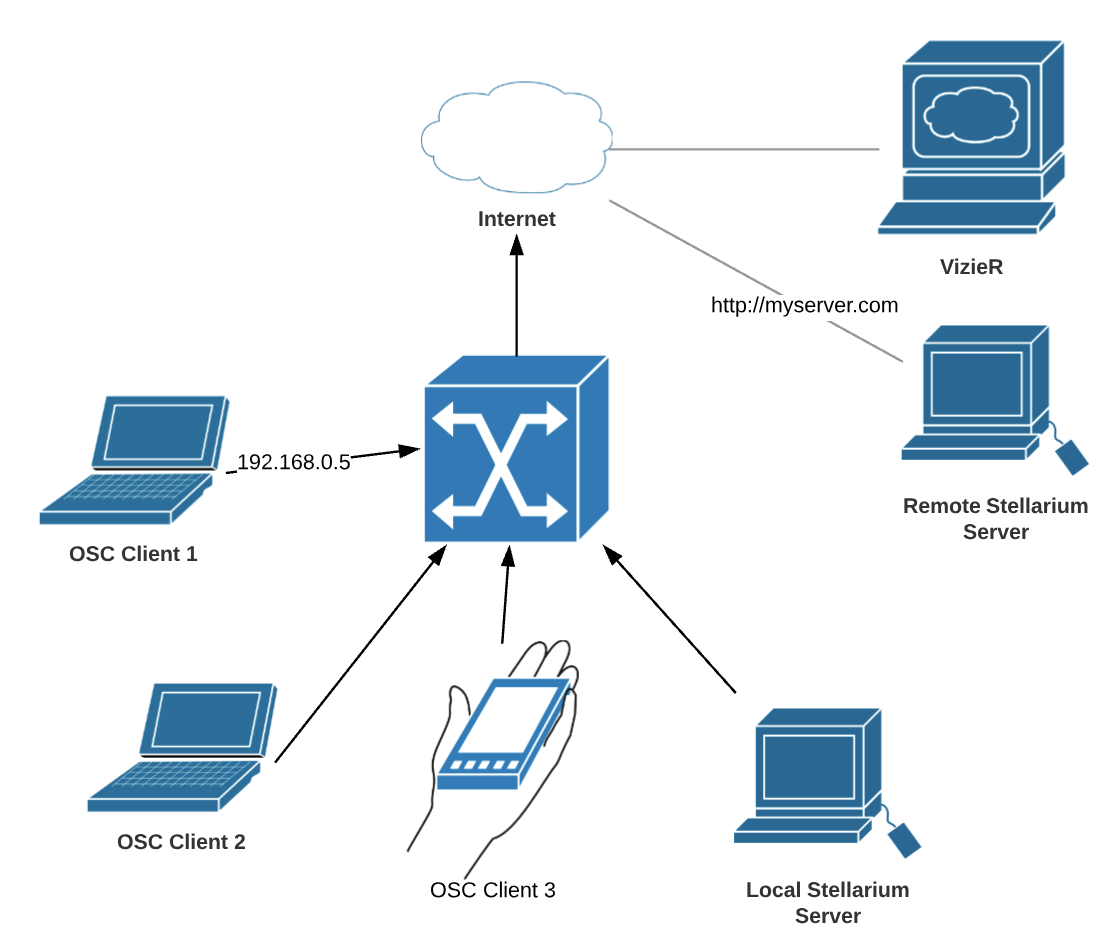
\includegraphics[width=1\columnwidth]{RemoteStellarium}
	\caption{Remote Stellarium and OSC Clients.}
	\label{fig:RemoteStellarium}
\end{figure}
\bigskip

Creating a connection between \textit{OSC Client 1} and \texttt{Remote Stellarium Server} is effected by adding adding the arguments \\\texttt{client=192.168.0.5} and \texttt{stellarium=http://myserver.com} to the command line.
This will cause the Stellar Command module to send OSC messages to ``192.168.0.5" and Stellarium commands to \textit{http://myserver.com} on HTP port 8090\footnote{The default Stellarium Remote Control port is 8090, however, this can be changed inside Stellarium. It is assumed that port forwarding when not using a local area network has been configured to send packages to the correct computer hosting Stellarium}, effectively acting as a proxy between the two.

   \begin{syntax}
	\medskip
	java -jar StellarCommand.jar port=1234 osc=/Stellar  {\char'134}\\client=192.168.0.5 stellarium=http://myserver.com\\
	\medskip
\end{syntax}
\bigskip

\clearpage
\pagestyle{ruled}

%#% extstart include laying-out-page.tex


\chapter{Laying out the page} \label{chap:layingpage}


    
\chapter{Comments}
\label{cha:comments}

\section{Algorithms}
\label{sec:algorithms}

Over time we may use this section to explain, or list some of the
algorithms for some of the macros in the class. The information may be
useful to some.

\subsection{Autoadjusting
  \texorpdfstring{\cs{marginparwidth}}{\textbackslash marginparwidth}}
\label{sec:auto-csmarg}

This algorithm is used within \cmd{\fixthelayout} unless the user have
used \cmd{\setmarginnotes}.

\noindent
\begin{framed}
  \vskip-2\baselineskip
  \begin{small}
\begin{verbatim}
if twocolumn then
  marginparwidth = min{inner margin,outer margin}
else
  if twoside then
    if marginpar always left or always right then
      marginparwidth = min{inner margin,outer margin}
    else if marginpar in outer margin then
      marginparwidth = outer margin
    else if marginpar in inner margin then
      marginparmargin = inner margin
    end if
  else
    if marginpar in left margin then
      marginparwidth = inner margin
    else
      marginparwidth = outer margin
    end if
  end if
end if
marginparwidth = marginparwidth - 2marginparsep
if marginparwidth < 1pt then
  marginparwidth = 1pt
end if
\end{verbatim}
  \end{small}
\end{framed}


%#% extend

%#% extstart input backend.tex


%%%%%%%%%%%%%%%%%%%%%%%%%%%%%%%%
%%\endinput
%%%%%%%%%%%%%%%%%%%%%%%%%%%%%%%

%%%%%%%%% end mbooka
%%%%%%%%%%%%%%%%%%%%%%%%%%%%%%%%%%%%%%%%%%%%%%%%%%%%%%%%%%%%

% back end
\backmatter

\PWnote{2009/07/08}{Changed \cs{toclevel@section} so that Notes 
                    divisions appear in the bookmarks}
\makeatletter\renewcommand*{\toclevel@chapter}{-1}\makeatother 
\makeatletter\renewcommand*{\toclevel@section}{0}\makeatother
\clearpage
\printpagenotes
\clearpage
\pagestyle{plainmarkruled}
%%\chapterstyle{section}

\renewcommand*{\begintheglossaryhook}{\small}
%%%\glossaryintoc
\printglossary

\renewcommand{\prebibhook}{%
\ctan\ is the \cTeXan. Information on how to
access CTAN is available at \url{http://www.tug.org}.
\par\vspace{\onelineskip}}

%%%\begin{comment}
\nocite{*}
\bibliographystyle{abbrv}

\bibliography{NIME_2019-planetarium} 


\clearpage
\twocolindex
\pagestyle{index}
%\renewcommand{\chaptermark}[1]{}
\renewcommand{\preindexhook}{%
The first page number is usually, but not always, the primary reference to
the indexed topic.\vskip\onelineskip}
\indexintoc

%%%\raggedright  does nasty things to index entries
\printindex

\onecolindex
\renewcommand*{\preindexhook}{}
\renewcommand*{\indexname}{Index of first lines}
%%% \indexintoc


\makeatletter
\renewcommand{\doidxbookmark}[1]{{\def\@tempa{Symbols}\def\@tempb{#1}%
  \centering\bfseries \ifx\@tempa\@tempb %
  Analphabetics 
%  \phantomsection%
%  \pdfbookmark[0]{Analphabetics}{Analphabetics-idx}%
%  \label{AnalphabeticsAnalphabeticsAnalphabetics-idx}%
  \else 
  #1%
%  \phantomsection%
%  \pdfbookmark[0]{#1}{#1-idx}%
%  \label{#1#1#1-idx}%
  \fi%
  \vskip\onelineskip\par}}
\makeatother


\printindex[lines]

\cleardoublepage
\pagestyle{empty}
\null\vfil

\begin{adjustwidth}{1in}{1in}
\begin{center}
{\Large\textsf{Colophon}}
\end{center}
\begin{center}
This manual was typeset using the \ltx\ typesetting system
created by Leslie Lamport and the \Mname\ class. 
The body text is set 10/12pt on a
33pc measure with Palatino designed by Hermann Zapf, which includes 
italics and small caps. Other fonts include
Sans, Slanted and Typewriter from Donald Knuth's 
Computer Modern family.

\end{center}


\end{adjustwidth}





\vfil

%#% extend


\end{document}

\endinput


%%% Local Variables: 
%%% mode: latex
%%% TeX-master: t
%%% TeX-source-specials-mode: t
%%% TeX-PDF-mode: t
%%% End: 
